%%%%%%%%%%%%%%%%%%%%%%%%%%%%%%%%%%%%%%%%%%%%%%%%%%%%%%%%%%%%%%%%%%%%%%%%%%%%%%%%%%%%%
% Machine Learning in Monitoring
%
% 1. Anomaly detection
%  - Adaptive using classifier updates
% 2. Alarm management
%  - Adaptive using RL
% 
%%%%%%%%%%%%%%%%%%%%%%%%%%%%%%%%%%%%%%%%%%%%%%%%%%%%%%%%%%%%%%%%%%%%%%%%%%%%%%%%%%%

ML prediction applications are effective complements to existing infrastructure in the process industry through soft sensors, state estimation, and forecasting. However, they are limited in applications regarding safety and risk management.  In the process industry, safety is upheld as the greatest \textit{value}; investing in a successful safety system is just good business.  

\begin{quote}
    "Safety is a \textbf{value}, not a priority.  Priorities change, but company values never do." \\
    --- Rex Tillerson, ex-CEO of ExxonMobil
\end{quote}

Decades ago, process safety investments are frowned upon by management due to its high costs and \textit{invisible} returns. In fact, construction workers used to cheer when project supervisors announced that \textit{only} 20 deaths will incur for this project---an event completely unacceptable in today's standards. Indeed, a perfect safety and risk management system results in \textit{no change} in day-to-day activities because all the incidents are proactively mitigated. As such, it is incredibly easy to become complacent towards risk management. However, if safety takes a back seat, the occurrence of the next incident is not a matter of if, its a matter of \textit{when}. Therefore, safety must be proactively (not reactively) managed to safeguard people, the environment, company assets, and production capabilities in terms of physical equipment and the social license to operate. Here, ML can be leveraged to proactively monitor process systems and create an additional layer of safety. In this chapter, ML algorithms will be applied to detect and predict equipment failures, process abnormalities, process variability and also perform alarm management. Through these applications, ML will be used to create multi-variate alarm systems that explore multi-variable interaction effects and gives fewer false alarms. Additionally, a new alarm management system that specifically tackles alarm flood scenarios will be introduced.  The objectives of this system are twofold: 1) Reduce sheer number of alarms during a flooding scenario; 2) identify the most important alarms so operators can prioritize safety critical alarms.

This chapter is organized as follows: Section 1 introduces data pre-processing methods for anomaly detection/prediction applications where the data is heavily imbalanced.  Section 2 introduces the anomaly detection and prediction algorithms and section 3 concludes this chapter with an introduction to a novel approach for alarm management.

The main contributions of this chapter are the data pre-processing methods used to prepare data sets for anomaly detection/prediction.  Additionally, it was shown that using synthetic data was able to enhance accuracy.  Lastly, a novel alarm management approach based on reinforcement learning was introduced to filter nuisance alarms and sort alarms based on their priority.  


\section{Data Pre-processing for Monitoring}
Data containing anomalous and/or incident events are extremely rare---thankfully---in the process industry. \begin{quote}
    Anomaly or anomalous activity: An abnormal or unexpected event given other variables (often multivariate).  For example, a person walking in a t-shirt when it is -$\ang{30}$ C outside.
\end{quote}

In fact, it is not uncommon to have just one incident in a data set containing hundreds of thousands of records.  Under such circumstances, building ML models to identify incidents is extremely difficult.  Remember, ML models are nothing more than statistical models with training formulated in an incremental updating fashion. In the scenario where the training data set contains 999,999 non-anomalous activities with 1 anomalous activity, the model will simply learn to return non-anomalous for all inputs; such a model would still achieve 99.9999\% accuracy on the training data!  When a human is provided with this data set, the human would instead focus most of its attention on the one anomalous activity, studying how it is different from all the other points.  A \textit{tabula rasa} machine is simply not equipped with such cognitive abilities, and will treat every data point equally; however, humans can artificially provide cognition to the machine.

\subsection{Data Prep for Anomaly Detection}
Anomaly \textit{detection} tasks are quite simple compared to anomaly \textit{prediction} tasks that will be discussed later on in this section. In anomaly detection, the model simply has to classify if there is an anomaly at current time. For example, given some states of a reactor, is the output temperature anomalous? That is, is the measured output temperature expected given the states?  Of course, such questions are difficult for humans to answer, especially in multi-variate environments; however, such questions can easily be answered by machines. Unfortunately, the events that are of interest to us (anomalies) are, often times, significantly more rare compared to normal process data. Hence, the leading reason for poor model performance in imbalanced data sets (i.e., distribution of different classes are vastly different) is the \textit{imbalanced} nature.  There exists two traditional ways to tackle the data imbalance issue: \textbf{undersampling} and \textbf{oversampling} \cite{under_over_sampling}.  Objectively, both methods aim to re-balance the data set so that the positive and negative data are in harmony.

A visual description of undersampling and oversampling is shown in Figure \ref{fig:03under_over_sampling}. In undersampling, the majority class(es) are significantly down-sampled to be the same size as the minority class.  The obvious flaw with this technique is the significant data in-efficiency.  In this method, the majority of the data that may contain critical features and information are simply discarded.  To take advantage of the whole data set, oversampling is sometimes used.  In oversampling, the minority class data is copied $n$ times until is approximately equivalent to the majority class.  Although oversampling allows the whole data set to be used, the models built typically overfit to the minority data simply because it was copied so many times.  During deployment, anomalies that are even slightly different from the ones in the training minority data set are often times misclassified.

Another more mathematical way to tackle this data imbalance issue is to bias the cost function to \textbf{heavily} discourage misclassification of positive samples.  However, such a methods requires tuning of the cost function, and is often times difficult.

\begin{figure}[H]
    \centering
    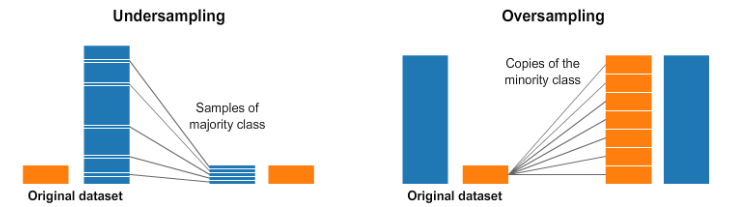
\includegraphics[width=0.8\textwidth]{images/ch3/over_and_undersampling.jpeg}
    \caption{A visual representation of undersampling (left) and oversampling (right). Original image from Kaggle.}
    \label{fig:03under_over_sampling}
\end{figure}

Luckily, normal process data are typically plentiful and lack "increasing" information (i.e., data is typically from steady state processes that hover around the same value for weeks) in the process industry.  Therefore, discarding large bulks of data in certain processes do not affect the ultimate accuracy of the model.  For anomaly detection, the majority class data was first undersampled to be comparable to the minority class. Undersampling should uniformly sample the data set to ensure all operating regimes are sufficiently captured. Then, a label column is generated; all anomalous events were given a value of 1 and normal process data had labels of 0.  An example of undersampling is shown below.  In this example, the process is deemed anomalous when $x_1 + x_2 > 3$.

\begin{table}[H]
    \centering
    \begin{tabular}{ c | c | c }
        $x_1$ & $x_2$ & label \\
        \hline
        2 & -1 & 0 \\
        3 & 0 & 0 \\
        2 & 5 & 1 \\
        2 & -2 & 0 \\
        5 & -1 & 1 \\
        -2 & -1 & 0 \\
        1 & -3 & 0 \\
        2 & -4 & 0 \\
        -2 & 2 & 0 \\
        -2 & 4 & 0 \\
    \end{tabular}
    \caption{Original data set before undersampling.}
    \label{tab:03undersampling}
\end{table}

Notice that in Table \ref{tab:03undersampling}, the majority class dominates the minority class 5:1.  After downsampling, the data set becomes:

\begin{table}[H]
    \centering
    \begin{tabular}{ c | c | c }
        $x_1$ & $x_2$ & label \\
        \hline
        2 & 5 & 1 \\
        2 & -2 & 0 \\
        5 & -1 & 1 \\
        -2 & -1 & 0 \\
    \end{tabular}
    \caption{Original data set before undersampling.}
    \label{tab:03undersampling2}
\end{table}
Note that the majority and minority class do not have to be perfectly balanced, especially in cases where perfectly balancing the classes require discarding unique information from the majority class.

\subsection{Data Prep. for Anomaly Prediction}
A visual breakdown of the anomaly prediction task is shown in Figure \ref{fig:03anomaly_pred}. From Figure \ref{fig:03anomaly_pred}, the \textit{old event} refers to the anomaly detection problem. The \textit{new event} denotes the latest time step to predict an anomalous event. Overall, anomaly prediction is a much more difficult problem compared to anomaly detection.  In anomaly prediction, the model must \textit{predict} if an anomaly is going to happen \textit{before} it happens.  Compared to anomaly detection, this task is much more difficult, and how far in advance an anomaly can be detected is heavily dependent on the speed of dynamics of the system.  For example, in cat classification, anomaly detection simply has to identify if the picture is a cat or not.  However, anomaly prediction has to predict if the animal in each picture will eventually grow up to become a cat.

\begin{figure}[H]
    \centering
    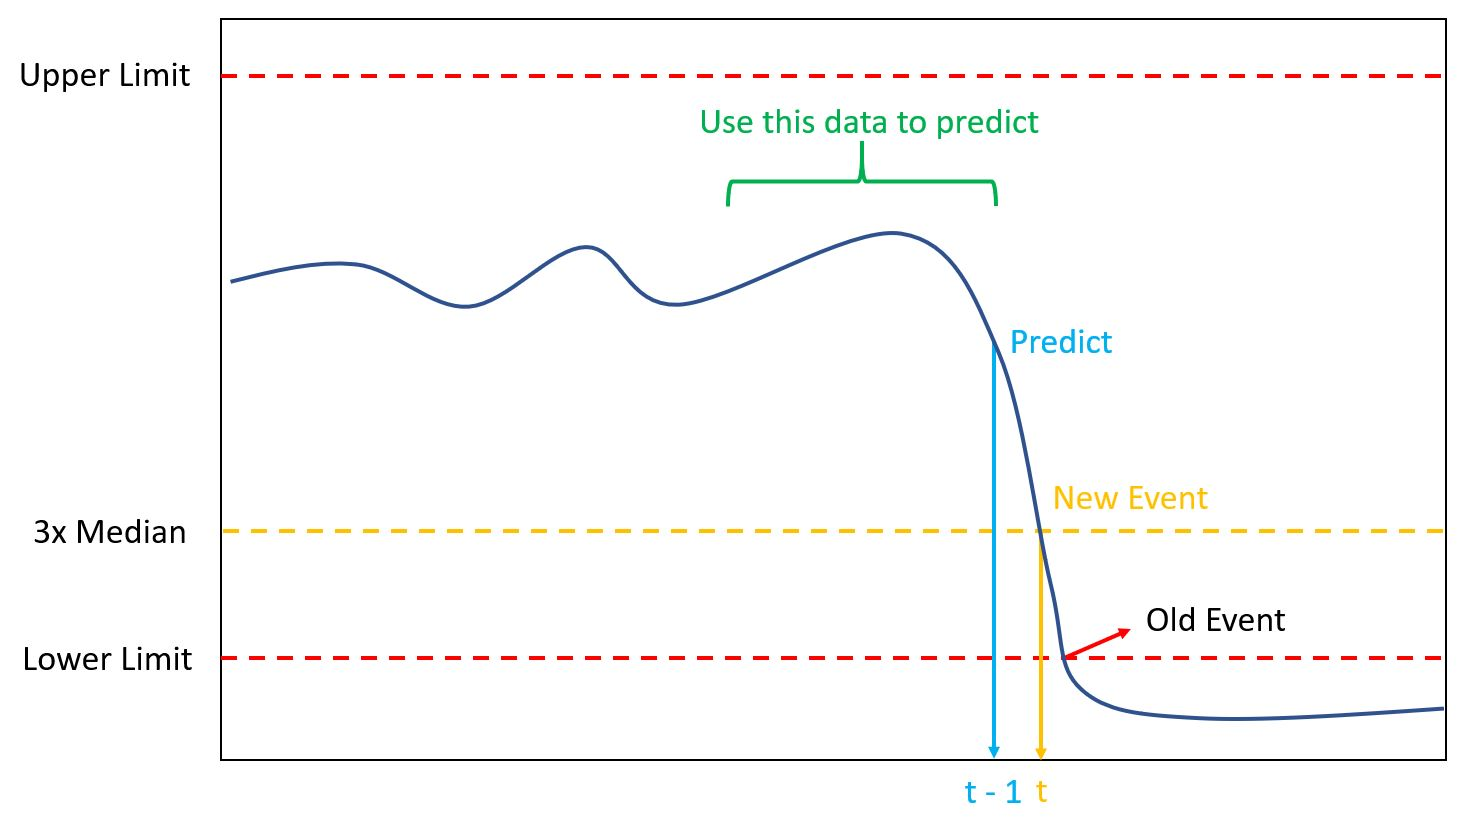
\includegraphics[width=0.9\textwidth]{images/ch3/anomaly_prediction.JPG}
    \caption{Visualization of the anomaly prediction.}
    \label{fig:03anomaly_pred}
\end{figure}

In anomaly prediction, the data is first labelled as in anomaly detection. Afterwards, the data is augmented as follows:
\begin{equation}
    x = [x_{t - l - L}, ...,  x_{t - l - 3}, x_{t - l - 2},  x_{t - l - 1},  x_{t - l}]
    \label{eq:03prediction}
\end{equation}
where $l > 0$ denotes the minimum number of sampling time the model should predict in advance.  $L$ represents the amount of previous information to be provided to the model. Augmenting the data as such provides temporal information to the ML algorithms to perform more accurate predictions. Note that even though an $l$ of 10 is chosen, this does not guarantee that the model will always predict anomalies 10 time steps in advance. Moreover, if the model predicts positive, it does not mean that an anomaly will occur exactly 10 time steps later. Merely, it just biases the algorithm to be more effective around that specific time range. How early an anomaly can be detected is purely dependent upon the dynamics of the system.  For example, if the degradation of an equipment is slow and gradual, the anomaly might be detected days in advance; however, an instantaneous failure offers no time for any early detection.

Like in anomaly detection, the data is heavily skewed towards normal process data; therefore, the majority class must also be downsampled to be comparable to the minority data set. Downsampling occurs last to ensure no temporal relationships are broken. A quantitative example for the augmentation of an anomalous data is shown below.  Here, suppose downsampling is not required (since an example is already shown above) and $l = 1; L = 2$.

\begin{table}[H]
    \centering
    \begin{tabular}{ c | c | c }
        $time$ & $x_2$ & label \\
        \hline
        0 & 5 & 0 \\
        1 & 3 & 0 \\
        2 & 7 & 0 \\
        3 & 6 & 0 \\
        4 & 4 & 0 \\
        5 & 2 & 0 \\
        6 & -1 & 1 \\
        7 & -3 & 0 \\
        8 & -1 & 0 \\
        9 & 2 & 0 \\
    \end{tabular}
    \caption{An arbitrary time-series data set.}
    \label{tab:03aug}
\end{table}

From Table \ref{tab:03aug}, the time series augmented data point for the anomalous event would be:
$$x = [x_3, x_4, x_5]$$
$$x = [6, 4, 2]$$


\subsection{Synthetic Data Generation}
In the above methods, the assumption of plentiful data was made.  In industry, this is not always true, especially for the anomalous data.  Here, three different \textit{synthetic} data generation methods will be introduced, with each method generating fake, yet similar, minority class data.  This topic is an especially popular research topic for the computer vision field where good, labeled data are rare. In fact, many "Completely Automated Public Turing test to tell Computers and Humans Apart" (CAPTCHAs) use traffic signs to force potential users of the website to first label some data, before being allowed to proceed. Most likely, the labeled data are then sold to computer vision companies. The main idea of synthetic data generation is to construct fake data that is \textit{exactly equivalent} to the real data that even a subject matter expert cannot tell them apart.  Indeed, that was exactly the structure of one of the most advanced generative methods, the generative adversarial network (GAN) \cite{gan}. Here, a generative neural network Synthetic data research in time-series data are unfortunately more primitive compared to GANs, but still provide valuable accuracy gains in the final model. 

\subsubsection{Time-series oversampling}
The first method caters to time-series data. This method simply oversamples the data leading up to an event.  Notice that this method is different from oversampling because it does not directly copy the data.  Instead, the sampling rate is increased for periods leading up to an anomalous event (for anomaly prediction) or during the anomalous event (for anomaly detection).  For example, the normal sampling time of a process might be one per minute. But to obtain more data, the resolution might be greatly enhanced to one per 10 seconds to increase anomalous data.

\subsubsection{SMOTE}
The second method for synthetic data generation is the Synthetic Minority Over-sampling Technique (SMOTE). As a high level overview, SMOTE generates synthetic minority data through combining features of real minority data points. Suppose we plotted a 2-class data set with 2 features.  Most likely, data points corresponding to the two classes will be segregated (at least slightly).  To generate synthetic data on either class: 
\begin{enumerate}
    \item Start with an arbitrary point within that class
    \item Identify the distance between that point and it's closest neighbour (within the same class).  Typically, Euclidean distance is used for the distance metric and is given by:
    \begin{equation}
        d(p, q) = \sqrt{(p_1 - q_1)^2 + (p_2 - q_2)^2 + ... + (p_n + q_n)^2}
    \end{equation}
    where $p$ and $q$ denotes two arbitrary points belonging to the same class.  Here, $n$ denotes the total number of features for $p$ and $q$.
    \item Multiply the Euclidean distance by an arbitrary number, $r$, between 0 - 1.
    \item Place a new data point $r \times d$ from the original point
\end{enumerate}

A visual representation of SMOTE is shown in Figure \ref{fig:03smote}. For more information regarding SMOTE, see \cite{smote}.

\begin{figure}[H]
    \centering
    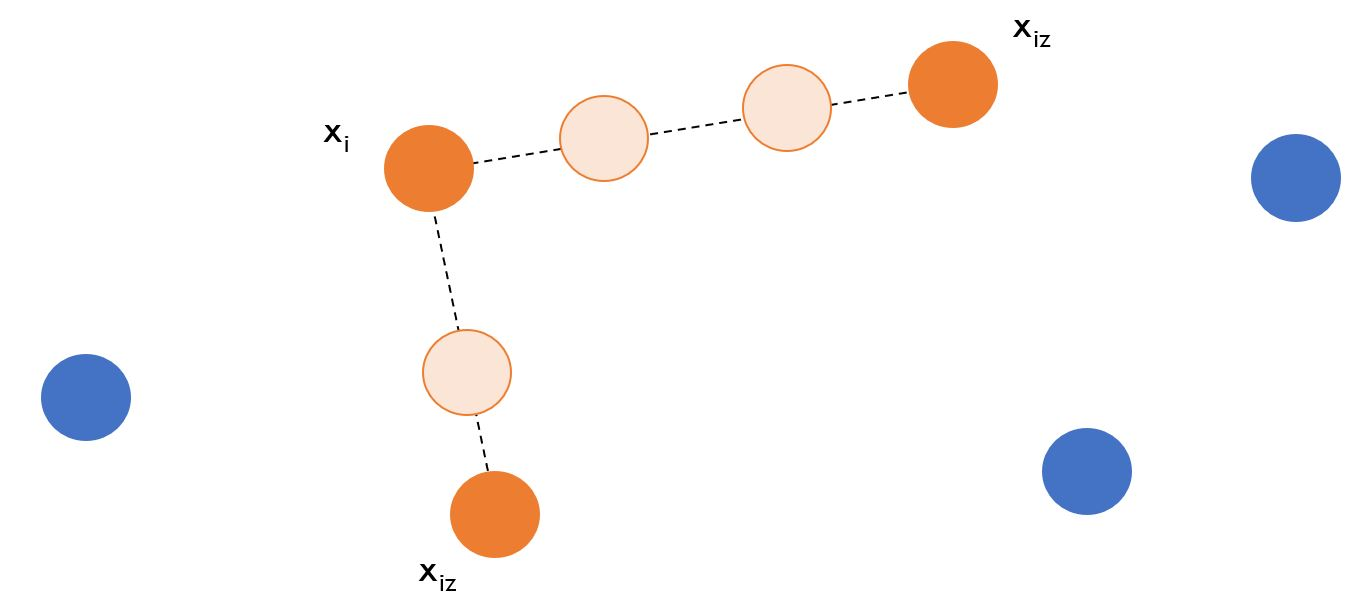
\includegraphics[width=0.9\textwidth]{images/ch3/smote.jpeg}
    \caption{A visual representation of SMOTE.}
    \label{fig:03smote}
\end{figure}

\subsubsection{ADASYN}
The last method is an adaptive version of SMOTE called ADASYN. ADASYN offers "targeted" data generation---more synthetic data is generated for neighbourhoods where the minority class is heavily dominated by the majority class.  For example, suppose the minority class is distributed into two distinct clusters, with one cluster having significantly more minority data compared to the other.  When training a ML model on such a data set, the model will perform significantly better on the minority-dense cluster.  ADASYN can be applied here to target more data generation on the less dense cluster, resulting in comparable model performance for both clusters.  However, ADASYN does not work for sparsely distributed minority classes where only one data point is present.  Additionally, some less dense clusters are a result of noise.  When ADASYN is applied on such clusters, inaccurate minority data will be created which greatly decrease model accuracy during deployment. A more detailed explanation of ADASYN can be found in \cite{adasyn}.


\section{Anomaly Detection and Prediction}
One of the simplest, yet very effective, classification machine learning algorithm is the logistic regression \cite{log_reg}. Logistic regression is a binary \textit{classification} algorithm (although called "regression") that outputs a value between 0 - 1, denoting the probability of a certain event occurring.  For example, the output value to a logistic regression model trained on pump failure data denotes the probability of the pump failing. The model structure of the logistic regression is given as:
\begin{equation}
    \hat{y} = \frac{1}{1 + e^{-(W_1^Tx_1 + W_2^Tx_2 + ... + b)}}
    \label{eq:02LogS}
\end{equation}
where $e$ denotes the exponential operator.  For multi-class classification, softmax functions are typically used and are given by:
\begin{equation}
    y = \frac{e^{z_i}}{\sum\limits^k_{j=0}e^{z_j}}
    \label{eq:03softmax}
\end{equation}
where $z_i$ is given as:
$$z_i = W_{i, 1}^Tx_1 + W_{i, 2}^Tx_2 + ... + b_i$$
The dimensions of the parameter matrices are $W_{j \times k}$ and $b_{j \times 1}$.  Here, $j$ amd $k$ denote the number of classes and the number of features for each data point, respectively.  Lastly, softmax are typically used because the function is continuously differentiable, thus allowing for gradient methods to be viable.

\subsection{Deep Learning Classification and Prediction}
A deep learning binary classification model simply modifies the regression neural network (introduced in the neural networks basic section in Chapter 1) by replacing the last layer's activation function to a sigmoid function. More specifically, the following is the mathematical procedure of the regression neural network model:
\begin{center}
    $z^{[1]}_j = W^{[1]}x + b^{[1]}$ \\
    $a^{[1]}_j = ReLU(z^{[1]}_j)$ \\
    $z^{[2]}_j = W^{[2]}a^{[1]}_j + b^{[2]}$ \\
    $a^{[2]}_j = ReLU(z^{[2]}_j)$ \\
    ... \\
    $z^{[r]}_j = W^{[r]}a^{[r - 1]}_j + b^{[r]}$ \\
    $a^{[r]}_j = ReLU(z^{[r]}_j)$ \\
    $y = W^{[o]}a^{[r]}_j + b^{[o]}$ \\  
\end{center}
In classification, the last step is simply replaced with:
$$z = W^{[o]}a^{[r]}_j + b^{[o]}$$
\begin{equation}
    y = \frac{1}{1 + e^{-z}}
    \label{eq:03sigmoidact}
\end{equation}
For multi-class deep learning classification, the output activation layer is replaced with the softmax function given in Equation \ref{eq:03softmax}.

\subsection{Cost Function for Classification}
The classification models are trained using the following convex cost function:
\begin{equation}
    J = \frac{1}{N}\sum\limits^N_{i=1} y_i \cdot log(f(x_i)) + (1 - y_i) \cdot log(1 - f(x_i))
    \label{eq:03maxentropy}
\end{equation}
where $N$ denotes the total number of training data used for this update step (i.e., the size of the mini-batch).  Here, $y_i$ is the label of the $i^{th}$ training data and $f(x_i)$ is the probability output of the classification model.  Intuitively, the cost function penalizes incorrect misclassifications.  For example, if $y_i = 1$ and $f(x_i) = 1$, then the cost function would be zero.  Likewise, if $y_i = 1$ and $f(x_i) = 0$, the cost function would instead return 1.



\section{Model Performance Assessment}
Often times, accuracy (i.e., \% of times the model predicted accurately) is a poor performance metric for heavily imbalanced data sets.  For example, a model that only predicts false for a classification data set where 99\% of the data is false will still result in a 99\% accuracy even though the model has no predictive capabilities. In such data sets, \textbf{precision} and \textbf{recall} are more proper evaluations of model performance \cite{prec_recall}.

\textbf{Precision:} Percent of time the model successfully predicted a true positive and is given as:
\begin{equation}
    Precision = \frac{TP}{TP + FP}
\end{equation}
where $TP$ and $FP$ denotes the true and false positives, respectively. A model with poor precision results in excessive false alarms and lead to operator complacency quickly.  

\textbf{Recall:} Percent of total events detected, given as:
\begin{equation}
    Recall = \frac{TP}{TP + FP}
\end{equation}
A poor recall model misses many anomalous events.

Typically, there is a trade-off between precision and recall for traditional methods. This could be eliminated, to an extent, using deep learning models trained on a large repository of data \cite{deeplearning_course}.  An acceptable precision and recall depends on the particular application.  For example, highly safety critical systems would require a near perfect recall because even missing one event could lead to catastrophic damage; therefore, a degree of false alarms is acceptable.  On the other hand, safety non-critical applications may favor a high precision model where every alarm should be guaranteed to correspond to an actual event. In non-safety critical applications, false alarms may lead to operator complacency. There do exist models with both high precision and recall; however, such models require vastly more data to identify.



\subsection{Interpreting ML Models}
Another critical requirement of ML models is that it must provide \textbf{real value} to the operators.  The algorithms presented here create value in two ways: 1) Provide explainability to the models which can increase intuition and gain addition buy-in from project shareholders and potential users; 2) provide actionable recommendations to operators.  It is almost useless to tell the operators that the plant will blow up in 10 minutes if no details on how to avoid such a fate is not provided.

The model weights can be analyzed to provide explainability for the logistic regression model.

The explainability of neural networks are significantly more difficult compared to logistic regression.  Indeed, even providing a rough explanation is extremely difficult. Some simple approaches include permutation importance, partial dependence plots, and SHAP.  

\textbf{Permutation importance:} Permutation importance identifies the importance of each input feature to the ML model and is applied \textit{after} the model is identified.  In permutation importance, the columns of the features are shuffled, one at a time.  After each shuffle, the model is re-evaluated with  one incorrect feature data.  Here, if the model's performance significantly reduces after the shuffling of a feature, that shuffled feature is deemed to have high predictive power.  On the other hand, if the model performance is unaffected, then the shuffled feature is assumed to have little to no predictive power. This step is repeated for all features in the feature space. More details regarding permutation importance can be found in \cite{perm_imp}, an example of feature shuffling is shown in Figure \ref{fig:03perm_imp}.
\begin{figure}[H]
    \centering
    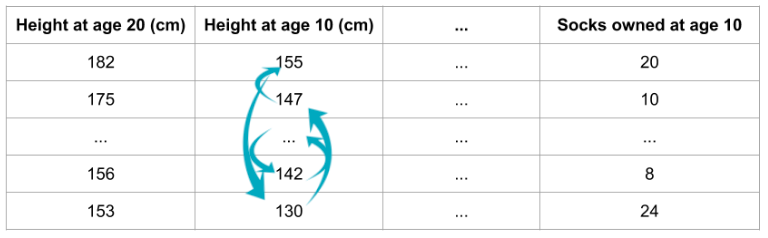
\includegraphics[width=0.8\textwidth]{images/ch3/perm_imp.jpeg}
    \caption{A visual example of permutation importance. Original image from \cite{img_perm_imp}.}
    \label{fig:03perm_imp}
\end{figure}


\textbf{Partial dependence plots:} Partial dependence plots (PDPs) are also evaluated after a model is identified and are used to show how each feature affects the final model prediction.  On a high level, PDPs are similar to evaluating the weights of the models, except PDPs also capture additional, more complex, relationships.  Basically, the fitted model is used to predict for the output while keeping all variables constant except for one.  

Figure \ref{fig:03pdp} shows an example of a PDP plot for one variable.  The y-axis shows the change in the prediction (in this case, winning "Player of the Game" in soccer) while the x-axis is the number of goals scored. Here, the number of goals scored is the variable being manipulated. The plot shows how the chance of winning "Player of the Game" changes as more goals are scored by a player.  In this particular example, the PDP shows that scoring one goal helps tremendously in obtaining player of the game; however, any additional goals provide no impact. For more information on PDPs, see \cite{pdp}.

\begin{figure}[H]
    \centering
    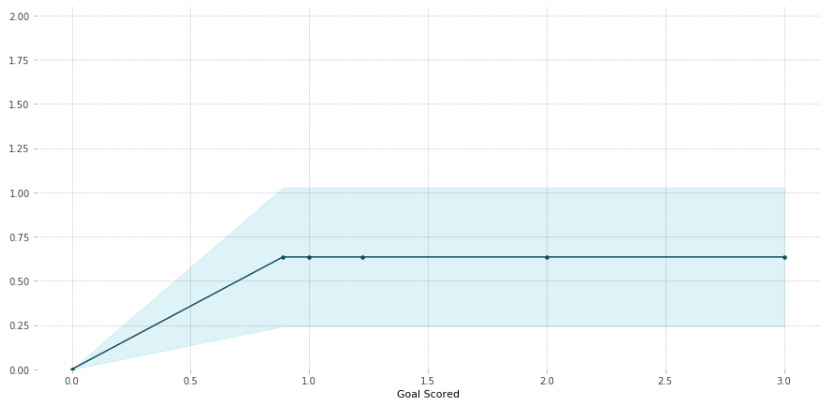
\includegraphics[width=0.8\textwidth]{images/ch3/pdp.jpeg}
    \caption{A visual example of permutation importance. Original image from \cite{pdp_plot}.}
    \label{fig:03pdp}
\end{figure}


\textbf{SHAP:} Shapley additive explanations (SHAP) are used to decompose model predictions so that the impact factor of each variable on the final prediction can be identified.  This analysis is critical for safety-sensitive systems; by applying SHAP, positive anomaly predictions can be decomposed to identify the root case (i.e., which feature is causing this prediction to be positive).  Overall, SHAP provide values that interprets the impact of having different values for certain features compared to if that feature took a baseline value.  For example, PDPs show how different the prediction would be, given a change in one variable. Instead, SHAP shows how the prediction is affected if one variable was changed, compared to if that variable took some baseline value.  In a multi-feature problem, a SHAP value is calculated from:
\begin{equation}
    y_{shap} = \sum y - y_{baseline}
    \label{eq:03SHAP}
\end{equation}
That is, the difference between what was predicted from the actual variable and what would have been predicted if a baseline value was used. The sum of all individual SHAP values correspond to how different the predicted value is from the baseline. Afterwards, a SHAP decomposition graph, as shown in Figure \ref{fig:03SHAPFig}, can be generated to explain exactly how the prediction was constructed.  Figure \ref{fig:03SHAPFig} was originally generated to predict the \% chance of winning the "Player of the Game" award in a soccer match.

\begin{figure}[H]
    \centering
    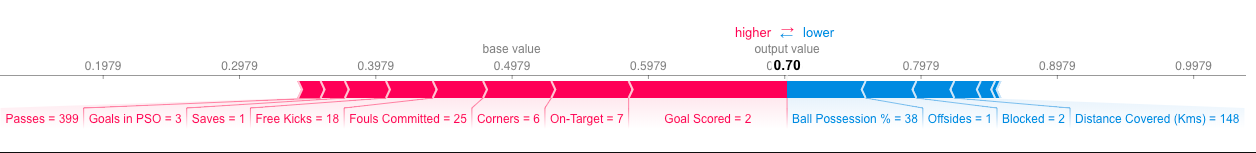
\includegraphics[width=0.99\textwidth]{images/ch3/SHAP.jpeg}
    \caption{A visual example of permutation importance. Original image from \cite{SHAP_plot}.}
    \label{fig:03SHAPFig}
\end{figure}

From Figure \ref{fig:03SHAPFig}, the red and blue arrows represent variables that resulted in a higher and lower chance of winning the "Player of the Game' award. For example, it can be seen that scoring two goals increased the chances of winning the award drastically; however, the ball possession being at 38\% reduced the chances. A more detailed description of SHAP can be found in \cite{SHAP}.




\section{Industrial Application of ML Monitoring}
The above algorithms were implemented onto an industrial pipeline for monitoring of an unreliable VFD.  Often times, the VFD would trip. When the VFD trips, the output pressure of the VFD drops to near zero. Initially, plant managers just wanted to detect when the VFDs trip through anomaly detection.  For the second phase of the project, the managers wanted to manage the VFDs proactively; thus, anomaly prediction was used predict \textit{in advance} when the VFDs will trip. Furthermore, management wanted the largest contributors of the VFD trip.  

\subsection{Anomaly Detection}
In total, the data set contained 54 anomalous events in a span of one year (525,600 data points) and are shown in Figure \ref{fig:03anomalous_events}. Some anomalous events lasted up to a few days but most ended within a few hours. In total, approximately 15\% of the data was anomalous (any values dipping below the dashed red line). 

\begin{figure}[H]
    \centering
    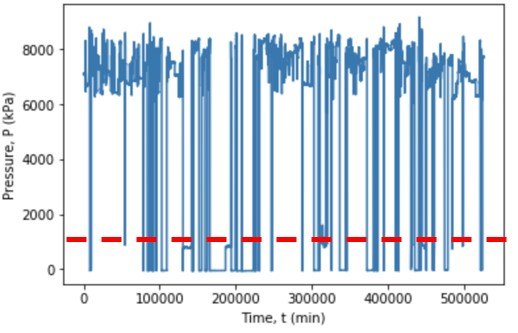
\includegraphics[width=0.7\textwidth]{images/ch3/anomalous_events.jpg}
    \caption{Anomalous events of a pump in an industrial pipeline.}
    \label{fig:03anomalous_events}
\end{figure}

The number of anomalous and non-anomalous data in the training and validation data sets are shown in Table \ref{tab:03train_validate}. In this study, an anomalous data is any point below the dashed red line shown in Figure \ref{fig:03anomalous_events}. For training and validation purposes, the data underwent a 90/10 split for the anomalous data.  In the end, 70,956 anomalous events were contained in the training data set and the remaining 7884 were in the validation data set. The data sets were then mixed with an equal number of non-anomalous data points.  No synthetic data generation methods were used here because there exists enough anomalous events to build an effective model.

\begin{table}[H]
    \centering
    \begin{tabular}{ c | c | c }
          & Anomalous & Non-anomalous  \\
        \hline
        Training & 70,956 & 70,956 \\
        Validation & 7884 & 7884 \\
    \end{tabular}
    \caption{Comparison of the best results achieved for anomaly detection and prediction.}
    \label{tab:03train_validate}
\end{table}

Data pre-processing followed similar methods as shown in Chapter 2 to initially reduce the number of redundant and/or unnecessary features.  The initial 785 input features were reduced to 64 following consulting with subject matter experts, redundancy analysis, and other analyses. Afterwards, logistic regression was applied onto the training data set.  The learning rate, mini-batch size, and number of training epochs for the model are 0.001, 256, and 800, respectively. The threshold for a positive classification was set at 0.5. Ultimately, the algorithm was able to achieve 99.6\% accuracy, 99.3\% precision, and 100\% recall on the training data.  The performance on the validation data was 99.7\% accuracy, 99.6\% precision, and 100\% recall.  From the results, it can be seen that deep learning was not required.

The largest contributors to the prediction model were:
\begin{enumerate}
    \item Motor Vibration
    \item Current Imbalance
    \item Ground Current
    \item Discharge Pressure
\end{enumerate}

Although the model above achieved high accuracy in detecting VFD trips, it is a reactive approach and does not prevent the incident from occurring.  Next, anomaly prediction algorithms will be shown where the events are predicted prematurely.  

\subsection{Anomaly Prediction}
Compared to anomaly detection, anomaly prediction is a much more difficult task.  Additionally, the amount of data present will be reduced tremendously.  That is, previously, there were approximately 78,840 anomalous data points; however, anomaly prediction can only use data right \textit{before} an incident occurs because its goal is to identify the dynamics behaviour of incidents before they occur.
Therefore, the total available data for anomaly prediction is only 54---the total number of events.

The anomaly prediction training and validation data also underwent a 90/10 split where 48 incidents were in the training data set and 6 incidents were in the validation data set. The data was then balanced with non-anomalous examples.  For the data augmentation, $l = 1$ and $L = 3$ (i.e., predict at least 1 step before the incident, and use the past 3 time step information for the prediction). The hyper parameters of the logistic regression were identical to those used in anomaly detection.

Table \ref{tab:03anomaly_pred_results} shows the performance of the anomaly prediction algorithm using different parameters.  In the headings of Table \ref{tab:03anomaly_pred_results}, \textit{Syn. Data} represents the amount of synthetic generated data points using ADASYN.  Here, $1 \times$ means 48 additional synthetic examples ($1 \times$ the total incidents).  N:A Ratio denotes the normal to anomalous data ratio.  For example, a N:A ratio of 12:1 means that the normal data points outnumber the anomalous data points 12 to 1. From Table \ref{tab:03anomaly_pred_results}, it can be seen that the initial precision was extremely low. With the addition of more normal data points, the precision increased significantly without much reduction in recall.  By tuning solely the N:A ratio, the best results obtained were 58\% precision and 98\% recall. To further increase accuracy, ADASYN was used to generate synthetic data.  After applying ADASYN, the best results achieved increased to 81\% precision and 92\% recall; still a large gap to ideal performance.  

In further improve accuracy, a three layer deep learning classifier was used.  The learning rate, mini-batch size, and training epochs were set to be the same as the logistic regression.  Ultimately, the deep learning classifier was able to achieve both 100\% precision and recall.

\begin{table}[H]
    \centering
    \begin{tabular}{ c | c | c | c | c | c}
        Precision & Recall & Activation & Syn. Data & N:A Ratio & Algorithm\\
        \hline
        15\% & 98\% & 0.70 & 0 & 1:1 & Log. regression  \\
        30\% & 79\% & 0.95 & 0 & 1:1 & Log. regression  \\
        54\% & 96\% & 0.70 & 0 & 5:1 & Log. regression  \\
        56\% & 93\% & 0.82 & 0 & 5:1 & Log. regression  \\
        41\% & 38\% & 0.95 & 0 & 5:1 & Log. regression  \\
        40\% & 96\% & 0.70 & 0 & 8:1 & Log. regression  \\
        42\% & 92\% & 0.83 & 0 & 8:1 & Log. regression  \\
        58\% & 98\% & 0.70 & 0 & 10:1 & Log. regression  \\
        57\% & 92\% & 0.83 & 0 & 10:1 & Log. regression  \\
        53\% & 96\% & 0.70 & 0 & 12:1 & Log. regression  \\
        57\% & 96\% & 0.83 & 0 & 12:1 & Log. regression  \\
        54\% & 98\% & 0.70 & $1 \times$  & 10:1 & Log. regression  \\
        62\% & 92\% & 0.83 & $1 \times$ & 10:1 & Log. regression  \\
        75\% & 96\% & 0.70 & $5 \times$ & 10:1 & Log. regression  \\
        81\% & 92\% & 0.83 & $5 \times$ & 10:1 & Log. regression  \\
        100\% & 100\% & 0.5 & $5 \times$ & 5:1 & Deep learning  \\
    \end{tabular}
    \caption{Precision and recall of the anomaly prediction algorithm using different parameters.}
    \label{tab:03anomaly_pred_results}
\end{table}

An example of the prediction algorithm in action is shown in Figure \ref{fig:03anomaly_prediction}.  It can be seen that the algorithm predicted the incident approximately 11 minutes in advance. The short prediction window is due to the suddenness of the events in this study.

\begin{figure}[H]
    \centering
    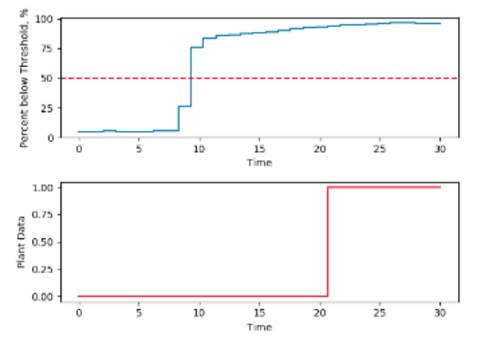
\includegraphics[width=0.6\textwidth]{images/ch3/an_pred.jpg}
    \caption{Anomaly prediction of an incident. Prediction algorithm output (top) as the incident gets closer (bottom).}
    \label{fig:03anomaly_prediction}
\end{figure}





















\section{Alarm Management}
Industry today is plagued with many problems that require advanced algorithms to overcome. Two of the largest problems are production optimization and alarm management. With continually pressure from environmental groups and ever-increasing government regulations, large industrial companies are forced to reduce their environmental footprints while improving output quality. The status quo also believes in zero-incident policies, i.e., all workplace incidents are preventable and unacceptable; therefore, it is in the best interest of the companies to implement effective, yet cheap, safety systems or their social license to operate could be compromised. To tackle these issues, the University of Alberta's process control team applied artificial intelligence (AI) algorithms in conjunction with classical approaches to an industrial scale wastewater treatment plant (WWTP) \footnote{This project was funded in part through an engage program with NTwist.}. The objectives were threefold: i) Design self-learning and adaptive RL controllers to seek out optimal operating strategies. In this case, the controllers must identify the optimal policy to meet government regulations in the most energy efficient way; ii) direct adaptive control, allowing the RL controller to learn optimal operating strategies as the operating conditions change by adapting the policy directly (not model re-identification since some systems may be unidentifiable), i.e. adapting to changes in season, new government regulations, etc; iii) superior alarm management by developing state-of-the-art alarm reduction and prioritization algorithms through pattern recognition and communication establishment between RL and the alarm system. Objectives 1 and 2 will be discussed in Chapter 4, objective 3 will be discussed in the following subsections.

Traditionally, alarms were the first line of defense against abnormalities in chemical processes, and were very effective \cite{alarm_manage}. Due to their cost of implementation, many teams of engineers and subject matter experts would gather together to brain storm the most effective alarm strategies. However, today's plants are littered with thousands of alarms due to the price of alarms plummeting after the invention of digital alarms. And because of their sheer number, many alarms are redundant and convey no additional information. 
This project aims to firstly reduce the amount of alarm floods through suppression and pattern recognition. Secondly, an alarm prioritization algorithm will be introduced so operators can focus their attention on the highest impact alarms first.

\subsection{System Description}
Figure \ref{fig:03WWTP} shows a schematic diagram of the WWTP.  A dynamic model of the WWTP was first built using the Benchmark Simulation No.1 documentation from the International Water Association \cite{wwtp}.  The WWTP comprises of a five-compartment activated sludge reactor and a ten-stage gravity separator.  The first two compartments of the reactor are anoxic tanks, the last three compartments are aerobic tanks.  The two control strategies are:

\begin{itemize}
	\item Manipulating the oxygen transfer coefficient $(K_La_5)$ to control the dissolved oxygen level in tank 5 
	\item Manipulating the internal recycle flow rate $(Q_a)$ to control the nitrogen level in tank 2
\end{itemize}

\begin{figure}[H]
    \centering
    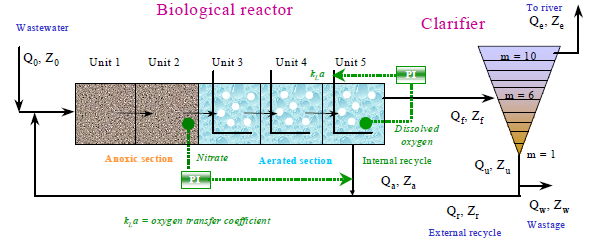
\includegraphics[width=0.85\textwidth]{images/ch3/WWTP.png}
    \caption{Schematic of the WWTP process. Original image from \cite{wwtp}.}
    \label{fig:03WWTP}
\end{figure}

The WWTP contains 145 states, 2 control actions, and 14 disturbances.  The states describe the characteristics of the overall WWTP system and contain process variables such as the flow rate and product compositions.  There are three sets of disturbances available to the WWTP: i) Dry weather data. ii) Rain weather data. iii) Storm weather data.  The results presented here use the dry weather data. For more detailed information regarding the WWTP, please refer to the Benchmark Simulation No.1 documentation \cite{wwtp}.

There exists five environmental constraints on the process:
\begin{enumerate}
    \item Total nitrogen ($N_{tot}$)
    \item Chemical oxygen demand (COD)
    \item $NH_4^+ + NH_3$ nitrogen ($S_{NH}$)
    \item Total suspended solids (TSS)
    \item Biochemical oxygen demand (BOD)
\end{enumerate}
The threshold for the environmental constraints is given as follows:
\begin{equation}
    Alarm = 
    \begin{cases}
    On,              & N_{tot}  > 10 \\
    On,              & COD  >  100 \\
    On,              & S_{nh} >  4 \\
    On,              & TSS > 30 \\
    On,              & BOD > 10 \\
    \end{cases}
    \label{eq:03constraints}
\end{equation}
If any of the above constraints are violated, an alarm will sound.

\subsection{Basics of Alarms}
In simple terms, alarm management is a special case of fault detection problem. Let $f_i \in \mathcal{F}$ be a set of possible faults and $A_i \in \mathcal{A}$ be a set of possible alarms.  On a high level, $f_i \rightarrow A_i$.  That is, all alarms are generated by some fault or some sequences of faults. In alarm management, the objective is reversed.  That is, $A_i$ is given, and the fault, $f_i$, that caused $A_i$ must be identified instead.

In industrial processes, alarm floods are mostly caused by chattering and redundant alarms or by poor alarm threshold design \cite{alarm_manage}. Chattering alarms often occur on noisy process variables. Here, the measurement(s) repeatedly violate the alarm limits purely due to measurement noise and do not pose any threat to the operation.  Redundant alarms refer to ones that repeat the same information as previous alarm.  For example, placing two alarms on a pipeline in series will cause the second alarm to be redundant because any process upsets will already be reported by the first alarm. Furthermore, many alarms are just poorly designed and contain extremely low thresholds; thus, activating even when no process upsets are present.  Given that thousands of alarms may be triggered at once, the prioritization of different alarms is equally difficult.  In this study, alarm reduction methods based on pattern recognition and RL will first be introduced.  Then, an alarm prioritization method on RL will be shown.

\subsection{Alarm Reduction}
The first algorithm in the SMART alarm management system is alarm reduction. Here, two methods will be proposed: 1) Alarm sequencing based on pattern recognition; 2) Alarm suppression via RL.

\subsubsection{Alarm Sequencing}
The first alarm reduction algorithm is called alarm sequencing.  The main goal is to create a sequence dictionary comprising of alarms that often occur (temporally) together \cite{alarm_sequence}.  For example, if alarms 1 and 2 frequently occur one after another, an alarm sequence, \emph{Sequence 1}, could be generated representing alarms 1 and 2. During an alarm flooding scenario, operators would see sequence 1 rather than alarms 1 and 2. In this simple scenario, the number of alarms appearing in the console would be halved.  More significant reduction in alarms can be achieved if 10 or 100 alarms often occur together.  The steps for the alarm reduction algorithm during initial set-up and online implementation is shown in Table \ref{alg:03AlarmReduce}.

\clearpage
\begin{table}[H]
    {\setstretch{1.2}
	\centering
	\begin{tabular}{p{14cm}}
	\hline
	\emph{Alarm Reduction Algorithm} \\
	\hline
	\textbf{Alarms from Plant} \\
	\hspace{0.5cm} Receive process alarms (typically as integers) \\
	\textbf{Alarm Coupling} \\
	\hspace{0.5cm} \textbf{Initialize} alarm combinations list \\
	\hspace{0.5cm} Group all alarms in pairs \\ 
	\hspace{1cm} \textbf{Save} grouped alarms in list \\
	\hspace{0.5cm} Group all alarms in triplets \\
	\hspace{1cm} \textbf{Save} grouped alarms in list \\
	\hspace{0.5cm} ... \\
	\hspace{0.5cm} \textit{Repeat until all alarms are grouped into one} \\
	\textbf{Sequence Identifier} \\ 
	\hspace{0.5cm} Count amount of times each \textbf{sequence} occurred \\
	\textbf{Sequence Dictionary Generation} \\
	\hspace{0.5cm} Initialize sequence dictionary \\
	\hspace{0.5cm} \textbf{If} group alarm occurred $\geq$ \emph{n} \\
	\hspace{1cm} Add grouped alarm to sequence dictionary \\
	\hspace{0.5cm} Return \textbf{Sequence Dictionary} \\
	\\
	\textbf{Online Implementation} \\
	\hspace{0.5cm} Receive alarms from process\\
	\hspace{0.5cm} \textbf{Alarm Masking} \\
	\hspace{1cm} \textbf{Group} previous two alarms \\
	\hspace{1.5cm} Check sequence dictionary for match \\
	\hspace{1.5cm} \textbf{If match} \\
	\hspace{2cm} Replace previous two alarms with first alarm in sequence \\
	\hspace{1cm} \textbf{Group} previous three alarms \\
	\hspace{1.5cm} Check sequence dictionary for match \\
	\hspace{1.5cm} \textbf{If match} \\
	\hspace{2cm} Replace previous three alarms with with first alarm in sequence \\
	\hspace{1.5cm} ... \\
	\hspace{1.5cm} ... \\
	\hspace{1cm} \emph{Repeat until end of sequence dictionary} \\
	\hline
	\end{tabular}}
	\caption{Alarm reduction algorithm}
	\label{alg:03AlarmReduce}
\end{table}

During online implementation, the alarm sequences are masked with the \textit{first} alarm in the sequence because it typically corresponds to the \textit{root cause} of the entire alarm sequence \cite{alarm_sequence}.  Moreover, simply displaying alarm sequences do little to help operators because it is essentially the same amount of alarms, except displayed in a more condensed format.

\subsubsection{Alarm Reduction through Suppression}
The second alarm reduction method suppresses low impact alarms altogether.  The algorithm starts by using RL to assign credits to different alarms via the optimal value or action-value functions, $v^*(x)$ and $Q^*(x, u)$, respectively.  During alarming events, alarms failing to exceed a threshold value will be suppressed and hidden from operators and is given mathematically by:
\[
    Alarm = 
\begin{cases}
    On,              & \text{if } v(x) < z \\
    Off,              & otherwise \\
\end{cases}
\]
where $z$ denotes some arbitrary threshold. Intuitively, this algorithm assesses each new alarm through observing the value of the current operating condition, $v(x)$. During critical events where alarms are necessary, $v(x)$ are intrinsically low because the plant would be operating far from ideal; however, during normal operations littered with nuisance alarms, $v(x)$ remains high resulting in suppression of all nuisance alarms.  This algorithm also acts as a \textit{multi-dimensional} alarm system.  That is, typical alarms occur after a higher or low limit is exceeded and do not consider multi-dimensional effects. By using the value functions of the process, the interaction effects can be additionally captured.

During initial identification of the $v(x)$ or $Q(x, u)$ values, both Markov reward processes (MRP) or Markov decision processes (MDP) can be used.  MRPs are used if only the alarm suppression algorithm is of interest and no actions are involved.  MDPs should be used if the plant managers also want to understand the optimal actions during different alarm events.  When using $Q(x, u)$, alarms are assigned the average $Q(x_i, u)$ for $x_i$ (i.e., average of $Q(x, u)$ across all possible actions).

Because $Q$-values may have significantly different magnitudes depending on the reward function design, the $Q$-values are first normalized using:
\begin{equation}
    Q_{i, norm} = \frac{Q_i - Q_{ave}}{\sigma}
\end{equation}
where $\sigma$ denotes the standard deviation of the $Q$-values.  In tabular cases, the mean and standard deviation of the $Q$-values can be found trivially because all $Q$-values are shown in the $Q$-table; however, deep RL approaches may face challenges.  One recommended solution would be to discretize the system and calculate the corresponding $Q$-values for each set of states and actions.  For example, suppose there exists a SISO system with $x \in [0, 5]$ and $u \in [5, 10]$.  The states and actions can be discretized as: $x = [0, 1, 2, 3, 4, 5]; u = [5, 6, 7, 8, 9, 10]$ and the average $Q$-values can be calculated as:
\begin{equation}
    Q_{ave} = \frac{1}{p \times q} \sum_{i, j = 0}^{p, q} Q(x_i, u_j | \theta)
    \label{eq:03mean_q}
\end{equation}
where $x_i$ and $u_j$ are the $i^{th}$ and $j^{th}$ state and action, respectively. Moreover, the standard deviation can be calculated as:
\begin{equation}
    \sigma = \sqrt{\frac{\sum (Q_i - Q_{ave})^2}{p \times q}}
    \label{eq:03sd_q}
\end{equation}

By normalizing the $Q$-values, the alarm threshold, $z$, across multiple units within a plant will share similar magnitudes and can be tuned easier.  Tuning of $z$ is dependent on the risk tolerance of the plant manager.  For a high amount of alarm suppression, $z$ can be tuned exceptionally low.  The steps to implementing this alarm reduction algorithm is as follows:

\begin{enumerate}
    \item Initialize the process and initialize the RL agent using any RL algorithm \textit{tabula rasa}.
    \item Allow RL to learn the value or action-values of the process through any traditional way (alarms are not required).
    \item After training, find the mean and standard deviations of the $Q$-values through Equations \ref{eq:03mean_q} and \ref{eq:03sd_q}.
    \item Online implementation: monitor alarms.  Any new alarm will be assigned the value or action-value at the time of their occurrence.  For alarm sequences, the assigned value is an exponentially weighted moving average (given in Equation \label{eq:08EWMA}) of the alarm values inside the sequence.  An EWMA was used because newer alarms matter more than old.
\end{enumerate}



\subsection{Alarm Prioritization}
During alarm flooding events, alarm reduction algorithms may reduce the amount of alarms to less than 5\% of total alarms.  However, it does not solve the root cause of the problem.  Also, 5\% of thousands of alarms is still far from useful and too much for a few operators to handle; therefore, a second algorithm was designed to sort the active alarms by a score.  Lower scores denote more dangerous alarms and will be placed on the top of the alarm log. Through this algorithm, the operators are equipped with knowledge regarding the priorities of different alarms and can work to resolve the safety critical ones first. 

The alarm prioritization algorithm is shown in Table \ref{alg:03alarmprioritization}.  On a high level, each alarm is assigned a value based on the current condition of the plant.  Alarms with higher values denote normal plant behaviour and are seen as unimportant.  Contrarily, alarms with low values correspond to poor plant performance; thus, alarms associated with low values may be critical.

\begin{table}[H]
    {\setstretch{1.2}
    \centering
	\begin{tabular}{p{13cm}}
	\hline
	\emph{Alarm Prioritization Algorithm} \\
	\hline
	\textbf{Alarms from Plant} \\
	\hspace{0.5cm} Receive process alarms (typically as integers) \\
	\hspace{0.5cm} Communication establishment with RL controller \\
	\hspace{1cm} Return value or average action-value in the given state \\
	\hspace{1cm} \textbf{If} new alarm is part of an existing sequence \\
	\hspace{1.5cm} Calculate the EWMA $Q$-value given previous values \\
	\hspace{1.5cm} Assign $Q$-value to alarm sequence \\
	\hspace{1cm} \textbf{Else} \\
	\hspace{1.5cm} Assign value or average action-value to the event \\
	\textbf{Alarm Sorting} \\
	\hspace{0.5cm}\textbf{While} value of new alarm is higher than alarm below \\
	\hspace{1cm} Move sequence down alarm log \\
	\hspace{0.5cm} \textbf{Return} sorted alarm log \\
	\hline
	\end{tabular}}
	\caption{Alarm prioritization algorithm.}
	\label{alg:03alarmprioritization}
\end{table}

Tables \ref{alg:03norm_system} and \ref{alg:03SMARTalarm} shows a comparison between a traditional alarm log compared to the proposed algorithm.  Comparing the alarm logs, it can be seen that the SMART alarm system was able to vastly reduce the amount of alarms, while putting the most important alarms on the top of the list. Additionally, the top alarm is comprised of a sequence of alarms.  The first alarm in the sequence (HH Vessel 2) is shown because it is assumed to be the root cause. Other alarms were not shown because their corresponding values are higher than the filtering threshold, $z$.  

\begin{table}[H]
	\centering
	\begin{tabular}{P{1.1cm}|P{2.1cm}|P{2.1cm}|P{2.5cm}|P{2cm}|P{2cm}}
	Events & Status & Date & Analysis & Value & Limit \\ \hline
	1 & Warning & March 22 & L Vessel 5 & 1.05 & 1.10 \\
	2 & Warning & March 22 & H Tank 2 & 61.2 & 60.0 \\
	3 & Warning & March 23 & L Vessel 3 & 0.96 & 1.15 \\
	4 & Alarm & March 23 & HH Tank 1 & 1.51 & 1.10 \\
	5 & Warning & March 23 & L Vessel 2 & 32.7 & 33.5 \\ 
	6 & Alarm & March 23 & HH Tank 3 & 40.2 & 33.5 \\
	\end{tabular}
	\caption{State-of-the-art industrial alarm system. L, H, LL, and HH corresponds to low, high, low low and high high levels.}
	\label{alg:03norm_system}
\end{table}

\begin{table}[H]
	\centering
	\begin{tabular}{P{2.5cm}|P{4.5cm}|P{2.5cm}|P{2.5cm}}
	Date & Status & Equipment &  Value\\ \hline
	March 22 & Alarm - Sequence & HH Tank 1 & 2.5\\
	March 23 & Warning & H Tank 2 &  9.5  \\
	March 23 & Warning & L Vessel 2 &  10.5 \\
	\end{tabular}
	\caption{SMART alarm system.}
	\label{alg:03SMARTalarm}
\end{table}

\subsection{Simulation Results}

The algorithms proposed above were simulated on the WWTP.  During training, the system was formulated as a MDP and the agent was trained for 10,000 episodes where each episode comprised of a 14 day period of dry weather.  Intuitively, the agent was trained for approximately 383.6 years in simulation time (2 hours physical time).  After training, the simulation was reset and the storm weather data was used.  The storm weather data was used because it is guaranteed to create many alarms in the system. In this study, warnings are triggered when values exceed 75\% of the constraints shown in Equation \ref{eq:03constraints}.  Moreover, alarms are triggered if the constraints are violated. To replicate a redundant alarming scenario, $S_{nh}$ alarms are placed on each stage of the separator; therefore, after one $S_{nh}$ alarm triggers, 9 additional alarms will follow due to redundancy.  Moreover, alarms are placed on the overall system to measure the other constraints as well.  To activate the alarm management system, the alarm sequence dictionary must first be built through pattern recognition.

The alarm sequence dictionary was first built by running the simulation once to identify common alarm sequences.  Alarm sequences were built based on the same alarm sequence happening more than 4 times.  Additionally, any alarms above $z = 0.5$ was filtered from the alarm log.  After $z$ and the alarm sequence dictionary were specified, the alarm management system was ready for use.  Two simulations were ran: one without the alarm management system and one with the alarm management system.

Without the system, there were 185 alarms generated within the process with no prioritization.  With the system, only 33 alarms were generated, resulting in a 82\% reduction in total alarms. Furthermore, the alarms were organized based on their priority.

The algorithms presented above are exploratory in nature and demonstrate the potential of RL in alarm management and root cause analysis problems. Here, three algorithms are presented to reduce and prioritize alarms with the assistance of RL. The presented algorithms have shown potential in a simple simulated example; however, have not been applied to large scale systems with thousands of alarms. One identifiable flaw with the sequencing technique is its space complexity.  In large industrial settings, there could exist millions of different sequences, rendering the method computational infeasible. To implement the alarm sequencing portion of this project, more research will be required.

